\documentclass[11pt]{beamer}  

\usetheme{Warsaw} 

%thèmes prédéfinis de Beamer 
%Antibes, boxes, classic, Darmstadt, Madrid
% Montpellier, Warsaw, Bergen, Berkeley, Goettingen, sidebar


%%%%%%%Tit\title{Titre principal}

\title[automatismes]{Automatismes en premi\'ere 2022/2023}
%\subtitle{Sous titre}
\author[F.Junier]{Fr\'ed\'eric Junier}
\institute[Le Parc]{{\centering Lyc\'ee du Parc \\
1 Boulevard Anatole France \\ 69006 Lyon }}
\date[\today]{\today}

\usepackage{etex}

%%%%%%%%%%%%Encodage du fichier source %%%%%%%%%%%
\usepackage[T1]{fontenc}
\usepackage[utf8]{inputenc}

\usepackage{lmodern}
\usepackage{url}
\usepackage[np]{numprint}


%%%%%%%%%%%%Là encore il y a de grosses différences entre le monde anglo-saxon et les francophones.Le séparateur des décimales est un point en anglais et une virgule en français. Leséparateur des milliers est une virgule en anglais et une espace insécable en français. Ilest préférable d’utiliser le package numprint (\usepackage{numprint}) qui associé àfrenchb produira la bonne typographie.
%123456789 = 123456789 \numprint{123456789} = 123 456 789  \numprint{3,1415926535897932384626} = 3,141 592 653 589 793 238 462 6  \numprint{12.34} = 12,34  En plus tu peux préciser les unités de cette façon : \numprint[kg]{12.34} = 12,34 kg ou encore \numprint[\degres C]{22} = 22°C Si tu veux utiliser le raccourci \np{} au lieu de \numprint{}, il te faut charger le package de cette façon : \usepackage[np]{numprint}


%%%%%%%%%%PSTricks%%%%%%%%%%%%

\usepackage{pstricks,pst-plot,pst-text,pst-tree,pst-eps,pst-fill,pst-node,pst-math,pstricks-add,pst-xkey,pst-eucl}


%%%%%%%Tikz%%%%%%%%%%%%%%%
\usepackage{pgf,tikz,tkz-tab}
% Pour les tableaux de signes ou de variations avec tkz-tab voir https://zestedesavoir.com/tutoriels/439/des-tableaux-de-variations-et-de-signes-avec-latex/#1-13389_tikz-un-package-qui-en-a-dans-le-ventre
\usetikzlibrary{arrows}
\usetikzlibrary{shapes.geometric}
\usetikzlibrary{shapes.geometric}
\usetikzlibrary{petri}
\usetikzlibrary{decorations}
\usetikzlibrary{arrows}
\usetikzlibrary{math}
 %Variables must be declared in a tikzmath environment but
       % can be used outside
%       \tikzmath{int \n; \n = 508; \x1 = 1; \y1 =1; 
%                   %computations are also possible
%                    \x2 = \x1 + 1; \y2 =\y1 +3; } 


%%%%%%%%%%%%%%%%%%%%%%%%%%%%%%%%%%%%%%%%
%%%%%%%%%%%Commandes Tikz Perso%%%%%%%%%%%%%%%

% Définition des nouvelles options xmin, xmax, ymin, ymax
% Valeurs par défaut : -3, 3, -3, 3
\tikzset{
xmin/.store in=\xmin, xmin/.default=-3, xmin=-3,
xmax/.store in=\xmax, xmax/.default=3, xmax=3,
ymin/.store in=\ymin, ymin/.default=-3, ymin=-3,
ymax/.store in=\ymax, ymax/.default=3, ymax=3,
}
% Commande qui trace la grille entre (xmin,ymin) et (xmax,ymax)
\newcommand {\grille}[2]
{\draw[help lines,black, thick] (\xmin,\ymin) grid[xstep=#1, ystep=#2] (\xmax,\ymax);}
% Commande \axes
\newcommand {\axes} {
\draw[->,very thick] (\xmin,0) -- (\xmax,0);
\draw[->,very thick] (0,\ymin) -- (0,\ymax);
\draw (0.95*\xmax, 0) node[above] {$x$};
\draw (0, 0.95*\ymax) node[left] {$y$};
}
% Commande qui limite l?affichage à (xmin,ymin) et (xmax,ymax)
\newcommand {\fenetre}
{\clip (\xmin,\ymin) rectangle (\xmax,\ymax);}

%Exemple d'utilisation

%\begin{center}
%\begin{tikzpicture} [xmin=-2,xmax=2,ymin=0,ymax=5]
%\grille{1} \axes \fenetre
%\draw plot[smooth] (\x,\x^2);
%\end{tikzpicture}
%\end{center}

%style pour la perspective cavalière française
%voir Tikz pour l'impatient page 68
\tikzset{math3d/.style=
{x= {(-0.353cm,-0.353cm)}, z={(0cm,1cm)},y={(1cm,0cm)}}}

%%%%%%%Symbole pour code calculatrice%%%%%%

%Flèche remplie pour défilement de menu

\newcommand{\flechefillright}{
\begin{tikzpicture}[scale=0.15] \fill (0,0)--(2,1)--(0,2)--cycle;
\end{tikzpicture}}

%%%%%%%%%%%%%Symboles pour calculatrice Casio%%%%
\newcommand{\execasio}{\Pisymbol{psy}{191}} %Retour chariot
\newcommand{\dispcasio}{\begin{pspicture}(.1,.1)\pspolygon*(.1,0)(.1,.1)\end{pspicture}} %Triangle « Disp »
\newcommand{\dispcasiotikz}{\begin{tikzpicture}[scale=0.2]
\fill (0,0) -- (1,0) -- (1,1) -- cycle;
\end{tikzpicture}} %Triangle « Disp »
%


%%%%%%%%%%%%%%%%%%%Présentation de codes sources%%%%%%%%%%%%%%%%%
\usepackage{listings}
%On utilise l?environnement lstlisting pour insérer
%un code source.
%En plus de l?environnement lstlisting, on peut également utiliser la
%commande \lstinline qui fonctionne comme la commande \verb, en ce
%sens qu?on peut utiliser n?importe quel caractère comme délimiteur. Enfin,
%la commande \lstinputlisting permet de charger un code source depuis
%un fichier externe.
%Il y a deux manières de préciser des options : soit via l?option de l?envi-
%ronnement ou de la commande, soit en utilisant la commande \lstset
%qui permet de définir des options de manière globale.

\lstset{ %
  language=Python,                % the language of the code
  basicstyle=\ttfamily,           % the size of the fonts that are used for the code
  %numbers=left,                   % where to put the line-numbers
  numberstyle=\tiny,  % the style that is used for the line-numbers
  %stepnumber=2,                   % the step between two line-numbers. If it's 1, each line 
                                  % will be numbered
  %numbersep=5pt,                  % how far the line-numbers are from the code
  backgroundcolor=\color{white},      % choose the background color. You must add \usepackage{color}
  showspaces=false,               % show spaces adding particular underscores
  showstringspaces=false,         % underline spaces within strings
  showtabs=false,                 % show tabs within strings adding particular underscores
  frame=single,                   % adds a frame around the code
  rulecolor=\color{black},        % if not set, the frame-color may be changed on line-breaks within not-black text (e.g. comments (green here))
  tabsize=4,                      % sets default tabsize to 2 spaces
  captionpos=b,                   % sets the caption-position to bottom
  breaklines=true,                % sets automatic line breaking
  breakatwhitespace=false,        % sets if automatic breaks should only happen at whitespace
  %title=\lstname,                   % show the filename of files included with \lstinputlisting;
                                  % also try caption instead of title
  breakindent=1cm,
  keywordstyle=\color{blue},          % keyword style
  commentstyle=\color{red},       % comment style
  %stringstyle=\ttfamily\color{green},         % string literal style
  escapeinside={\%*}{*)},            % if you want to add LaTeX within your code
  morekeywords={*,...},              % if you want to add more keywords to the set
  deletekeywords={...}              % if you want to delete keywords from the given language
  upquote=true,columns=flexible,
xleftmargin=1cm,xrightmargin=1cm,
 inputencoding=utf8,			%Les lignes qui suivent sont pour le codage utf8
  extendedchars=true,
  literate=%
            {é}{{\'{e}}}1
            {è}{{\`{e}}}1
            {ê}{{\^{e}}}1
            {ë}{{\¨{e}}}1
            {û}{{\^{u}}}1
            {ù}{{\`{u}}}1
            {â}{{\^{a}}}1
            {à}{{\`{a} }}1
            {î}{{\^{i}}}1
            {ô}{{\^{o}}}1
            {ç}{{\c{c}}}1
            {Ç}{{\c{C}}}1
            {É}{{\'{E}}}1
            {Ê}{{\^{E}}}1
            {À}{{\`{A}}}1
            {Â}{{\^{A}}}1
            {Î}{{\^{I}}}1
}

\lstdefinestyle{rond}{
  numbers=none,
  backgroundcolor=\color{gristclair},
  frameround =tttt
}

\lstdefinestyle{compil}{
  numbers=none,
  backgroundcolor=\color{gristclair}
}
%\lstset{language=Python,basicstyle=\small , frame=single,tabsize=4,showspaces=false,showtabs=false,showstringspaces=false,numbers=left,numberstyle=\tiny , extendedchars=true}

%%%%%%%%%%%AmsMaths%%%%%%
\usepackage{amsmath,amsfonts,amssymb}
\usepackage{pifont,fourier}
\usepackage{ bclogo}


%%%%%Commande \DeclareMathOperator pour définir de nouveaux opérateurs (en lettres romaines droites)%%%%%
%\DeclareMathOperator{\sh}{sh}
%\DeclareMathOperator{\ch}{ch}

%%%%%%%%%%%%%%%%%%Maths divers%%%%%%%%%%%%%%%%%%%%%%%%%
%Delimiteurs
\newcommand{\delim}[3]{\raise #1\hbox{$\left #2\vbox to #3{}\right.$}}


%%%%%%%%%%%%%Nombres%%%%%%%%%%%%%%%%

%Ensemble prive de...
%\newcommand{\prive}{\boi}%{\backslash}

%Ensembles de nombres%%%%%%%%%%%%%%%%%
\newcommand{\R}{\mathbb{R}}
\newcommand{\N}{\mathbb{N}}
\newcommand{\D}{\mathbb{D}}
\newcommand{\Z}{\mathbb{Z}}
\newcommand{\Q}{\mathbb{Q}}
\newcommand{\C}{\mathbb{C}}
\newcommand{\df}{~\ensuremath{]0;+\infty[}~}
\newcommand{\K}{\mathbb{K}}

%%%%%%%%Arithmetique%%%%%%%%%%
%PGCD, PPCM
\newcommand{\PGCD}{\mathop{\rm PGCD}\nolimits}
\newcommand{\PPCM}{\mathop{\rm PPCM}\nolimits}

%Intervalles
\newcommand{\interoo}[2]{]#1\, ;\, #2[}
\newcommand{\Interoo}[2]{\left]#1\, ;\, #2\right[}
\newcommand{\interof}[2]{]#1\, ;\, #2]}
\newcommand{\Interof}[2]{\left]#1\, ;\, #2\right]}
\newcommand{\interfo}[2]{[#1\, ;\, #2[}
\newcommand{\Interfo}[2]{\left[#1\, ;\, #2\right[}
\newcommand{\interff}[2]{[#1\, ;\, #2]}
\newcommand{\Interff}[2]{\left[#1\, ;\, #2\right]}
%\newcommand\interentiers #1#2{[\! [#1\, ;\, #2]\! ]}
\newcommand{\interentiers}[2]{\llbracket #1\, ;\, #2\rrbracket}
%


%%%%%%%%%%%%%%Nombres complexes%%%%%

\newcommand{\ic}{\text{i}}
%\newcommand{\I}{\text{i}}
\newcommand{\im}[1]{\text{Im}\left(#1\right)}
\newcommand{\re}[1]{\text{Re}\left(#1\right)}
\newcommand{\Arg}[1]{\text{arg}\left(#1\right)}
\newcommand{\Mod}[1]{\left[#1\right]}
%Parties entière, réelle, imaginaire, nombre i
\newcommand{\ent}[1]{\text{E}\left(#1\right)}
\renewcommand{\Re}{\mathop{\rm Re}\nolimits}
\renewcommand{\Im}{\mathop{\rm Im}\nolimits}
\renewcommand{\i}{\textrm{i}}

%%%%%%%%%%%Probabilites et statistiques%%%%%
\newcommand{\loibinom}[2]{\mathcal{B}\left(#1\ ; \ #2 \right)}
\newcommand{\loinorm}[2]{\mathcal{N}\left(#1\ ; \ #2 \right)}
\newcommand{\loiexp}[1]{\mathcal{E}\left(#1\right)}
\newcommand{\proba}[1]{\mathbb{P}\big(#1\big)}
\newcommand{\probacond}[2]{\mathbb{P}_{#2}\big(#1\big)}
\newcommand{\esperance}[1]{\mathbb{E}\left(#1\right)}
\newcommand{\variance}[1]{\mathbb{V}\left(#1\right)}
\newcommand{\ecart}[1]{\sigma\left(#1\right)}
\newcommand{\dnormx}{\frac{1}{\sqrt{2\pi}} \text{e}^{-\frac{x^2}{2}}}
\newcommand{\dnormt}{\frac{1}{\sqrt{2\pi}} \text{e}^{-\frac{t^2}{2}}}
\newcommand{\nbalea}[2]{\reinitrand[first=#1, last=#2, counter=num]  \rand $\thenum$}  %retourne un entier aleatoire antre les bornes #1 et #2 comprises
%Covariance
\newcommand{\cov}{\mathop{\rm cov}\nolimits}
%


%%%%%%%%%%Analyse%%%%%%%%%%%

%%%%%%%%%%%Courbe%%%%%%%%%%%%
\newcommand{\courbe}[1]{\ensuremath{\mathcal{C}_{#1}}}

%%%%%%%Fonction exponentielle%%%%%
\newcommand{\fe}{~fonction exponentielle~}
\newcommand{\e}{\text{e}}

%Fonction cotangente
\newcommand{\cotan}{\mathop{\rm cotan}\nolimits}
%%%%%%%%%%%%%%%%%%%%%%%%%%%%%%%%%%%%%%%%%
%
%Fonctions hyperboliques
\newcommand{\ch}{\mathop{\rm ch}\nolimits}
\newcommand{\sh}{\mathop{\rm sh}\nolimits}


%%%%%%%%%%%%%%Limites%%%%%%
\newcommand{\limite}[2]{\lim\limits
_{x \to #1} #2}
\newcommand{\limitesuite}[1]{\lim\limits
_{n \to +\infty} #1}
\newcommand{\limiteg}[2]{\lim\limits
_{\substack{x \to #1 \\ x < #1 }} #2}
\newcommand{\limited}[2]{\lim\limits
_{\substack{x \to #1 \\ x > #1 }} #2}

%%%%%%%%%%Continuité%%%%%%%%%%%
\newcommand{\TVI}{théorème des valeurs intermédiaires}

%%%%%%%%%%%Suites%%%%%%%%%%%%
\newcommand{\suite}[1]{\ensuremath{\left(#1_{n}\right)}}
\newcommand{\Suite}[2]{\ensuremath{\left(#1\right)_{#2}}}
%

%%%%%%%%%%%%%%%Calcul intégral%%%%%%
\newcommand{\dx}{\ensuremath{\text{d}x}}		% dx
\newcommand{\dt}{\ensuremath{\text{d}t}}		% dt
\newcommand{\dtheta}{\ensuremath{\text{d}\theta}}		% dtheta
\newcommand{\dy}{\ensuremath{\text{d}y}}		% dy
\newcommand{\dq}{\ensuremath{\text{d}q}}		% dq

%%%Intégrale%%%
\newcommand{\integralex}[3]{\int_{#1}^{#2} #3 \ \dx}
\newcommand{\integralet}[3]{\int_{#1}^{#2} #3 \ \dt}
\newcommand{\integraletheta}[3]{\int_{#1}^{#2} #3 \ \dtheta}

%%%%%Equivalent%%
\newcommand{\equivalent}[1]{\build\sim_{#1}^{}}

%o et O%%%%
\renewcommand{\o}[2]{\build o_{#1\to #2}^{}}
\renewcommand{\O}[2]{\build O_{#1\to #2}^{}}



%%%%%%%%%%%%%%%Geometrie%%%%%%%%%%%%%%%%%%%%%%%

%%%%%%%%%%%%%%%Reperes%%%%%%%%%%%%%%
\def\Oij{\ensuremath{\left(\text{O},~\vect{\imath},~\vect{\jmath}\right)}}
\def\Oijk{\ensuremath{\left(\text{O},~\vect{\imath},~ \vect{\jmath},~ \vect{k}\right)}}
\def\Ouv{\ensuremath{\left(\text{O},~\vect{u},~\vect{v}\right)}}
\renewcommand{\ij}{(\vec\imath\, ;\vec\jmath\,)}
\newcommand{\ijk}{(\vec\imath\, ;\vec\jmath\, ;\vec k\,)}
\newcommand{\OIJ}{(O\,;\, I\,;\, J\,)}
\newcommand{\repere}[3]{\big(#1\, ;\,\vect{#2} ;\vect{#3}\big)}
\newcommand{\reperesp}[4]{\big(#1\, ;\,\vect{#2} ;\vect{#3} ;\vect{#4}\big)}

%%%%%%%%%Coordonnees%%%%%%%%%%%%%%
\newcommand{\coord}[2]{(#1\, ;\, #2)}
\newcommand{\bigcoord}[2]{\big(#1\, ;\, #2\big)}
\newcommand{\Coord}[2]{\left(#1\, ;\, #2\right)}
\newcommand{\coordesp}[3]{(#1\, ;\, #2\, ;\, #3)}
\newcommand{\bigcoordesp}[3]{\big(#1\, ;\, #2\, ;\, #3\big)}
\newcommand{\Coordesp}[3]{\left(#1\, ;\, #2\, ;\, #3\right)}
\newcommand{\Vcoord}[3]{\begin{pmatrix} #1 \\ #2 \\ #3 \end{pmatrix}}
%Symboles entre droites
%\newcommand{\paral}{\sslash}
\newcommand{\paral}{\mathop{/\!\! /}}
%

%%%%%%%%%Produit scalaire, Angles%%%%%%%%%%
\newcommand{\scal}[2]{\vect{#1} \, \cdot \, \vect{#2}}
\newcommand{\Angle}[2]{\left(\vect{#1} \, , \, \vect{#2}\right)}
\newcommand{\Anglegeo}[2]{\left(\widehat{\vect{#1} \, ; \, \vect{#2}}\right)}
\renewcommand{\angle}[1]{\widehat{#1}}
\newcommand{\anglevec}[2]{\left(\vect {#1}\, ,\,\vect {#2} \right)}
\newcommand{\anglevecteur}[2]{(#1\, , \, #2)}
\newcommand{\Anglevec}[2]{(\vecteur{#1}\, ,\,\vecteur{#2})}
\newcommand{\prodscal}[2]{#1 \, \cdot \, #2}
%


%Arc
%\newcommand{\arc}[1]{\wideparen{#1}}
\newcommand{\arcoriente}[1]{\overset{\curvearrowright}{#1}}
%
%


%%%%%%%%%%%%%%%Normes%%%%%%%%%%%%%%%%
\newcommand{\norme}[1]{\left\| #1\right\|}
\newcommand{\normebis}[1]{\delim{2pt}{\|}{9pt}\! #1\delim{2pt}{\|}{9pt}}
\newcommand{\normetriple}[1]{\left |\kern -.07em\left\| #1\right |\kern -.07em\right\|}
\newcommand{\valabs}[1]{\big| \, #1 \, \big|}
%

%%%%%%%%%%%%%%%%%%%%%%%%%%%Degré%%%%%%
%\newcommand{\Degre}{\ensuremath{^\circ}}
%La commande \degre est déjà définie dans le package babel

%%%%%%%%%%Vecteurs%%%%%%%%%%%
\newcommand{\vect}[1]{\mathchoice%
{\overrightarrow{\displaystyle\mathstrut#1\,\,}}%
{\overrightarrow{\textstyle\mathstrut#1\,\,}}%
{\overrightarrow{\scriptstyle\mathstrut#1\,\,}}%
{\overrightarrow{\scriptscriptstyle\mathstrut#1\,\,}}}



%%%%%%%%%%%%%Algebre%%%%%%%%%%%%%%%


%%%%%%%%%%Systemes%%%%%%%%%%%
%Systemes
\newcommand{\sys}[2]{
\left\lbrace
 \begin{array}{l}
  \negthickspace\negthickspace #1\\
  \negthickspace\negthickspace #2\\
 \end{array}
\right.\negthickspace\negthickspace}
\newcommand{\Sys}[3]{
\left\lbrace
 \begin{array}{l}
  #1\\
  #2\\
  #3\\
 \end{array}
\right.}
\newcommand{\Sysq}[4]{
\left\lbrace
 \begin{array}{l}
  #1\\
  #2\\
  #3\\
  #4\\
 \end{array}
\right.}
%
%

%%%%%%%%%%%%%%%%Matrices%%%%%%%%%%%%%%%%%%
%Comatrice
\newcommand{\com}{\mathop{\rm com}\nolimits}
%
%
%Trace
\newcommand{\tr}{\mathop{\rm tr}\nolimits}
%
%
%Transposee
\newcommand{\transposee}[1]{{\vphantom{#1}}^t\negmedspace #1}
%
%
%Noyau
\newcommand{\Ker}{\mathop{\rm Ker}\nolimits}
%
%

%
%Matrices
\newcommand{\Mn}{\mathcal M_n}
\newcommand{\matrice}[4]{
\left(
 \begin{array}{cc}
  #1 & #2 \\
  #3 & #4
 \end{array}
\right)}

\newcommand{\Matrice}[9]{
\left(
 \begin{array}{ccc}
  #1 & #2 & #3\\
  #4 & #5 & #6\\
  #7 & #8 & #9
 \end{array}
\right)}
\newcommand{\Vect}[3]{
\left(\negmedspace
 \begin{array}{c}
  #1\\
  #2\\
  #3
 \end{array}\negmedspace
\right)}
\newcommand{\Ideux}{\matrice{1}{0}{0}{1}}
\newcommand{\Itrois}{\Matrice{1}{0}{0}{0}{1}{0}{0}{0}{1}}
%
%
%Determinants
\newcommand{\determinant}[4]{
\left|
 \begin{array}{cc}
  #1 & #2 \\
  #3 & #4
 \end{array}
\right|}
\newcommand{\Determinant}[9]{
\left|
 \begin{array}{ccc}
  #1 & #2 & #3\\
  #4 & #5 & #6\\
  #7 & #8 & #9
 \end{array}
\right|}

%%%%%%%%%%%%%%Calculs en Latex%%%%%%%%%%%%%

\usepackage[first=1,last=100]{lcg}  %%%%%%%générer des nombres pseudo aléatoires
%%%%
\usepackage{calc} %   pour faire des calculs%%


%%%%Mise en page%%%%%
\usepackage{fancybox}
\usepackage{lastpage}
\usepackage{hyperref}
%À mettre dans le préambule pour faire apparaitre le plan à chaque section 

\AtBeginSection[ ]
{
\begin{frame}<beamer>
\frametitle{Plan}
\tableofcontents[currentsection]
\end{frame}
}

%%%%%%%¨Puces%%%%%%%%%%%%
\usepackage{enumerate}


%%%%%%%%%%%%Graphiques%%%%%%%%%%%%%%
\usepackage{graphicx,pgf}				
\usepackage{pstricks,pst-plot,pst-text,pst-tree,pst-eps,pst-node,pst-math,pstricks-add}
 


%%%%%%Numérotation des automatismes%%%%%%
\newcounter{autocompteur}
\setcounter{autocompteur}{0}
\newcommand{\automatisme}[1]{\addtocounter{autocompteur}{1}\frametitle{Automatisme  \theautocompteur  \textit{ thème : #1}}}
%%%%%%%%%%%%%%%%%%%%%%%%%%%%%%%%%%%%%%%%%%%%%%%%

%%%%%%%%%%%%%%%Francisation%%%%%%%%%%%%%%
\usepackage[french]{babel}
\frenchbsetup{StandardLists=true}

%%%%%%%%%%%%%%%%%%%%%%%%%%%%%%%%%%%%%%%%%



\begin{document}

\frame{\titlepage}

\section{Calcul}



\begin{frame}
\automatisme{Puissances}


\begin{enumerate}
	\item Écrire $(3^{2} \times 3^{5})^{4}$ sous la forme d'une puissance de $3$.
	\item Soit $ABC$ un triangle rectangle en $A$ tel que $AB=5$ et $BC=13$, calculer la longueur $AC$.
	\item Simplifier $\left(2\sqrt{3}\right)^{4}$
	\item Simplifier $\frac{4+\sqrt{60}}{2}$
	\item Soit $a$ et $b$ des réels avec $b\geqslant 0$, simplifier $\frac{a-\sqrt{b}}{2}-\frac{-a+\sqrt{b}}{2}$
        \item Développer et réduire $\left(\frac{a+b+c}{2}\right)^{2}-\left(\frac{a+b-c}{2}\right)^{2}$
  \end{enumerate}
\end{frame}

 
\begin{frame}
\automatisme{Fractions}

Réduire au même dénominateur et simplifier les expressions suivantes définies pour l'indéterminée $x$ ou $n$.

\begin{itemize}
\item $\frac{1}{n}-\frac{1}{n+1}$
\item $\frac{1}{n-4}-n$
\item $\frac{1}{(n+1)^{2}}+\frac{1}{n+1}-\frac{1}{n}$
\item $\frac{x}{x-1}-\frac{2}{x+1}-\frac{2}{x^2-1}$
\item $\frac{1}{x} + \frac{x+2}{x^{2}-4}+\frac{2}{x^{2}-2x}$
\end{itemize}

\end{frame}





\begin{frame}
\automatisme{Factoriser}

Soit $a$ un réel.

\begin{itemize}
\item Factoriser $a^{4}-16$
\item Factoriser $a^2-1+3a-3$ par $a-1$
\item Factoriser $2a^2+5a+2$ par $a+2$
\item Factoriser $a^{2}+a-2$
\item Factoriser $a^{2}+a-6$
\end{itemize}

\end{frame}


\section{Second degré}


\begin{frame}
\automatisme{Résoudre une équation du second degré}


\begin{itemize}
\item Déterminer le nombre de solutions dans $\R$ de l'équation  $x^{2}=m$ si $m>0$
\item Déterminer le nombre de solutions dans $\R$ de l'équation  $x^{2}=m$ si $m=0$
\item Déterminer le nombre de solutions dans $\R$ de l'équation  $x^{2}=m$ si $m<0$
\item Résoudre mentalement dans $\R$ l'équation $x^{2}=9$
\item Résoudre mentalement dans $\R$ l'équation $(x-1)^{2}=9$
\item Résoudre mentalement dans $\R$ l'équation $16-(x-1)^{2}=7$
\end{itemize}

\end{frame}


\begin{frame}
\automatisme{Déterminer l'axe de symétrie d'une parabole}


\begin{itemize}
\item Déterminer l'axe de symétrie de la parabole d'équation $y=x^{2}$
\item Déterminer l'axe de symétrie de la parabole d'équation $y=3-x^{2}$
\item Déterminer l'axe de symétrie de la parabole d'équation $y=(x-3)^{2}$
\item Déterminer l'axe de symétrie de la parabole d'équation $y=(x+3)^{2}$
\item Déterminer l'axe de symétrie de la parabole d'équation $y=(3-x)^{2}-1$
\item Déterminer l'axe de symétrie de la parabole d'équation $y=-3x^{2}-6x+1$
\end{itemize}

\end{frame}


\begin{frame}
\automatisme{Déterminer les racines d'un trinôme}

Soit $a$ un réel.

\begin{itemize}
\item Déterminer les racines du trinôme d'expression $f(x)=-3(x+2)(1-x)$
\item Déterminer les racines du trinôme d'expression $f(x)=16-x^{2}$
\item Déterminer les racines du trinôme d'expression $f(x)=x^{2}+1$
\item Déterminer les racines du trinôme d'expression $f(x)=16-(x-1)^{2}$
\end{itemize}

\end{frame}



\begin{frame}
\automatisme{second degré}

Pour chacun des trinômes suivants déterminer le signe de son discriminant sans le calculer.
\begin{itemize}
\item $f_{1}$ définie sur $\R$ par $f_{1}(x)=x^2+100$
\item $f_{2}$ définie sur $\R$ par $f_{2}(x)=(x-100)^2$
\item $f_{3}$ définie sur $\R$ par $f_{3}(x)=(x+100)^2$
\item $f_{4}$ définie sur $\R$ par $f_{4}(x)=x^2-100$
\end{itemize}

\end{frame}



\section{Dérivation locale}

\label{derivationglocale}


\begin{frame}
\automatisme{dérivation locale}

Soit $f$ la fonction définie sur $\Interoo{-\infty}{0}$ par  $f(x)=\frac{1}{x}$.
\begin{itemize}
\item Soit un réel $a<0$ et un réel $h \neq 0$ tel que $a+h<0$, démontrer que $\frac{f(a+h)-f(a)}{h}=\frac{-h}{(a+h)a}$.
\item En déduire que $f$ est dérivable en tout réel $a<0$ et déterminer l'expression de $f'(a)$.
\item Déterminer une équation de la tangente à la courbe de $f$ au point d'abscisse $-2$.
\end{itemize}

\end{frame}


\section{Dérivation Globale}

\label{derivationglobale}

\begin{frame}
\automatisme{dérivation}

Déterminer une expression de la fonction dérivée pour la fonction $f$ dérivable sur l'intervalle I.
\begin{itemize}
\item $f:x \mapsto \frac{x^3-1}{5x^{2}+1}$ sur $\R$ ;
 \item $f:x \mapsto x^2\sqrt{x}$ sur $\Interoo{0}{+\infty}$ ;
 \item $f:x \mapsto \left(8-3x\right)^{7}$ sur $\Interoo{0}{+\infty}$ ; 
 \item $f:x \mapsto 4x-\frac{1}{x-3}$ sur $\Interoo{3}{+\infty}$.
\end{itemize}

\end{frame}

\begin{frame}

\automatisme{dérivation}

Soit $f$ une fonction dérivable sur $\Interff{-8}{6}$ dont on donne le tableau de variation ci-dessous.

%:-+-+-+-+- Engendré par : http://math.et.info.free.fr/TikZ/TableauxVariations/
\begin{center}
\begin{tikzpicture}[scale=0.5]
% Styles 
\tikzstyle{cadre}=[thin]
\tikzstyle{fleche}=[->,>=latex,thin]
\tikzstyle{nondefini}=[lightgray]
% Dimensions Modifiables
\def\Lrg{1.5}
\def\HtX{1}
\def\HtY{0.5}
% Dimensions Calculées
\def\lignex{-0.5*\HtX}
\def\lignef{-1.5*\HtX}
\def\separateur{-0.5*\Lrg}
% Largeur du tableau
\def\gauche{-1.5*\Lrg}
\def\droite{8.5*\Lrg}
% Hauteur du tableau
\def\haut{0.5*\HtX}
\def\bas{-1.5*\HtX-2*\HtY}
% Ligne de l'abscisse : x
\node at (-1*\Lrg,0) {$x$};
\node at (0*\Lrg,0) {$-8$};
\node at (2*\Lrg,0) {$-5$};
\node at (4*\Lrg,0) {$2$};
\node at (6*\Lrg,0) {$3$};
\node at (8*\Lrg,0) {$6$};
% Ligne de la fonction : f(x)
\node  at (-1*\Lrg,{-1*\HtX+(-1)*\HtY}) {$f(x)$};
\node (f1) at (0*\Lrg,{-1*\HtX+(0)*\HtY}) {$4$};
\node (f2) at (2*\Lrg,{-1*\HtX+(-1)*\HtY}) {$0$};
\node (f3) at (4*\Lrg,{-1*\HtX+(-2)*\HtY}) {$-1$};
\node (f4) at (6*\Lrg,{-1*\HtX+(-1)*\HtY}) {$0$};
\node (f5) at (8*\Lrg,{-1*\HtX+(0)*\HtY}) {$$};
% Flèches
\draw[fleche] (f1) -- (f2);
\draw[fleche] (f2) -- (f3);
\draw[fleche] (f3) -- (f4);
\draw[fleche] (f4) -- (f5);
% Encadrement
\draw[cadre] (\separateur,\haut) -- (\separateur,\bas);
\draw[cadre] (\gauche,\haut) rectangle  (\droite,\bas);
\draw[cadre] (\gauche,\lignex) -- (\droite,\lignex);
\end{tikzpicture}
\end{center}
%:-+-+-+-+- Fin

%:>>>>> code du tableau à ré-injecter
%[
%	["x", "f'(x)", "f(x)"],
%	["-8", "", "-", "4"],
%	["-5", "", "-", "0"],
%	["2", "", "+", "-1"],
%	["3", "", "+", "0"],
%	["6", "7", "?", ""]
%]

\begin{enumerate}
	\item Dresser le tableau de signes de la fonction dérivée $f'$ de $f$ sur l'intervalle $\Interff{-8}{6}$.
	
	\item Dresser le tableau de variations d'une fonction $F$ dérivable sur l'intervalle $\Interff{-8}{6}$ et dont la dérivée est $f$.
	
\end{enumerate}

\end{frame}



\begin{frame}
\automatisme{dérivation}

Déterminer une expression de la fonction dérivée pour la fonction $f$ dérivable sur l'intervalle I.
\begin{itemize}
\item $f:x \mapsto \sqrt{3x+1}$ sur $\Interoo{-\frac{1}{3}}{+\infty}$ ;
 \item $f:x \mapsto (5x-3)\sqrt{x}$ sur $\Interoo{0}{+\infty}$ ;
 \item $f:x \mapsto \left(605x-3\right)^{607}$ sur $\R$ ; 
 \item $f:x \mapsto \frac{1}{3}-\frac{2}{3-x}$ sur $\Interoo{3}{+\infty}$.
\end{itemize}

\end{frame}




\section{Suites numériques}



\begin{frame}
\automatisme{suites}


\begin{itemize}
\item Soit la suite $\suite{u}$ définie pour tout entier naturel $n$ par $u_{n}=n^{2}-n$. Calculer $u_{4}$ et $u_{7}$.
 \item Soit la suite $\suite{u}$ définie pour tout entier naturel $n$ par $u_{0}=4$ et $u_{n+1}=2u_{n}-1$. Calculer $u_{1}$, $u_{2}$ et $u_{3}$.
 \item Soit la suite $\suite{u}$ définie pour tout entier naturel $n$ par $u_{0}=1$ et $u_{n}=u_{n-1}-n+1$. Calculer $u_{1}$, $u_{2}$ et $u_{3}$.
\end{itemize}

\end{frame}


\begin{frame}[fragile]
\automatisme{suites}
\begin{lstlisting}
#On définit la suite (Un) par Un=f(n)
def f(n):
  if n==0:
    return 1
  else:
    return 1/n**2  
# n**2 signifie le carré de n
\end{lstlisting}

Interpr\'eteur en ligne : \url{https://repl.it/@Reformelycee/suite-explicite}.

\begin{itemize}
	\item $u_{0}=1$ Vrai ou Faux ?
	\item $u_{1}=0,5$ Vrai ou Faux ?
	\item $u_{50}=0,0004$ Vrai ou Faux ?
	\item La suite n'est pas d\'efinie en $0$. Vrai ou Faux ?
\end{itemize}
\end{frame}


\section{Application du produit scalaire}

\label{prodscalaire}

\begin{frame}
\automatisme{Application du produit scalaire}

\begin{center}
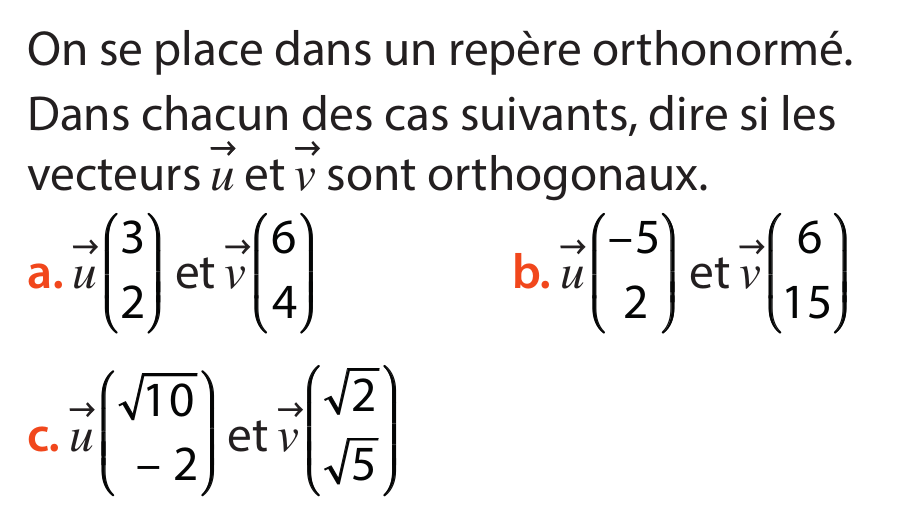
\includegraphics[scale=0.3]{ressources/prodscal-1.png}
\end{center}


\end{frame}


\begin{frame}
\automatisme{Application du produit scalaire}

\begin{center}
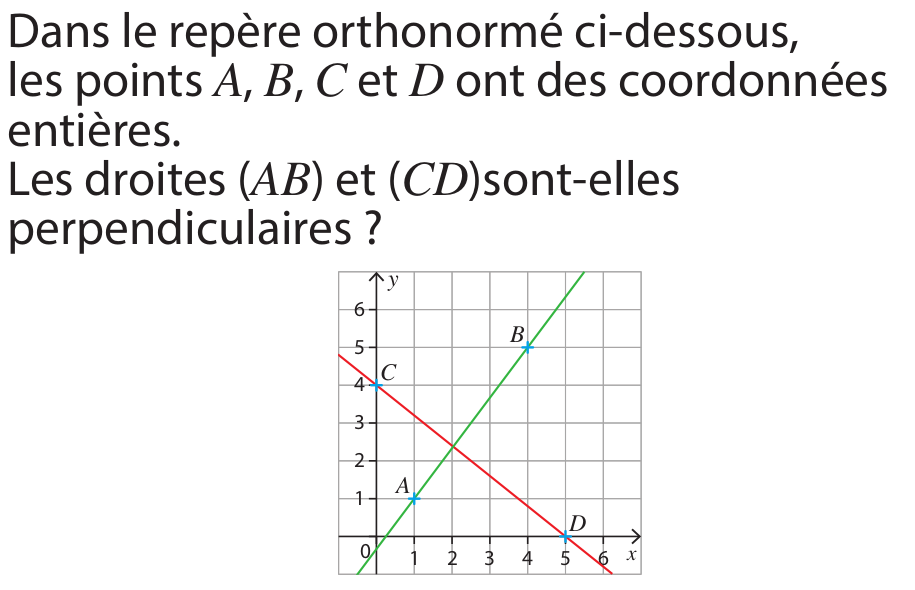
\includegraphics[scale=0.3]{ressources/prodscal-2.png}
\end{center}


\end{frame}


\begin{frame}
\automatisme{Application du produit scalaire}

\begin{center}
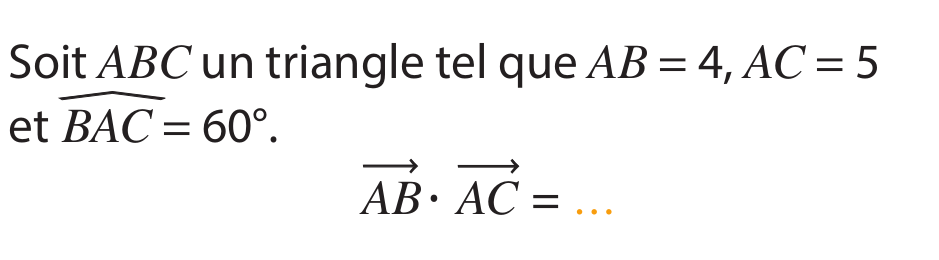
\includegraphics[scale=0.3]{ressources/prodscal-3.png}
\end{center}


\end{frame}


\begin{frame}
\automatisme{Application du produit scalaire}

\begin{center}
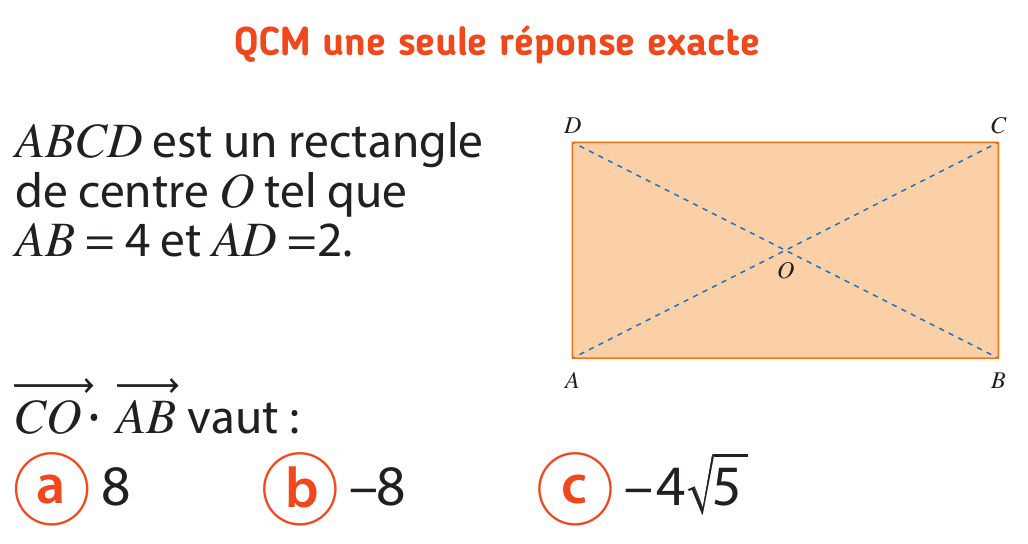
\includegraphics[scale=0.3]{ressources/prodscal-4.png}
\end{center}


\end{frame}


\begin{frame}
\automatisme{Application du produit scalaire}

\begin{center}
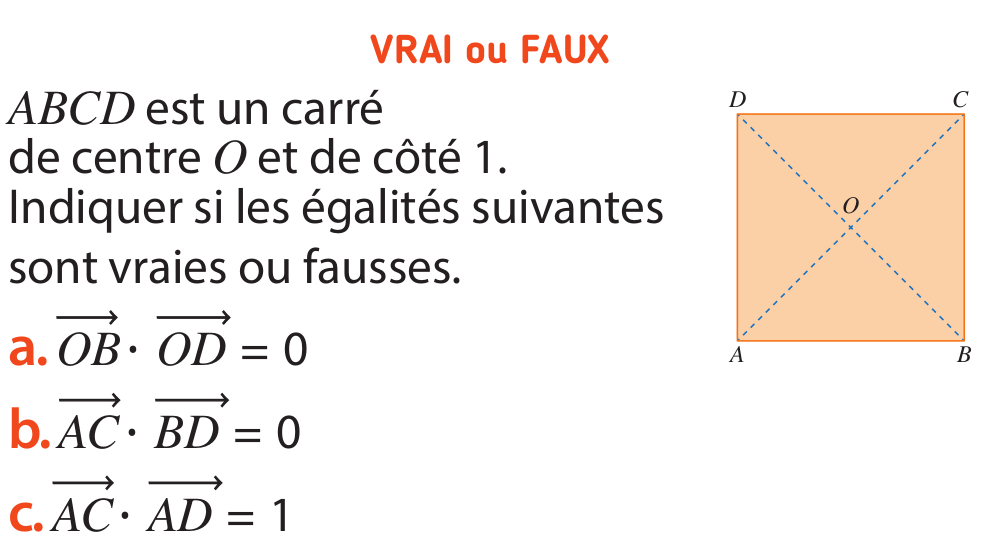
\includegraphics[scale=0.3]{ressources/prodscal-5.png}
\end{center}


\end{frame}


\begin{frame}
\automatisme{Application du produit scalaire}

\begin{center}
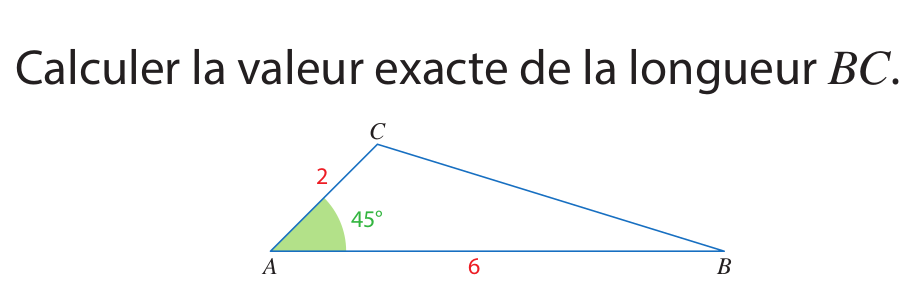
\includegraphics[scale=0.3]{ressources/prodscal-6.png}
\end{center}


\end{frame}


\begin{frame}
\automatisme{Application du produit scalaire}

\begin{center}
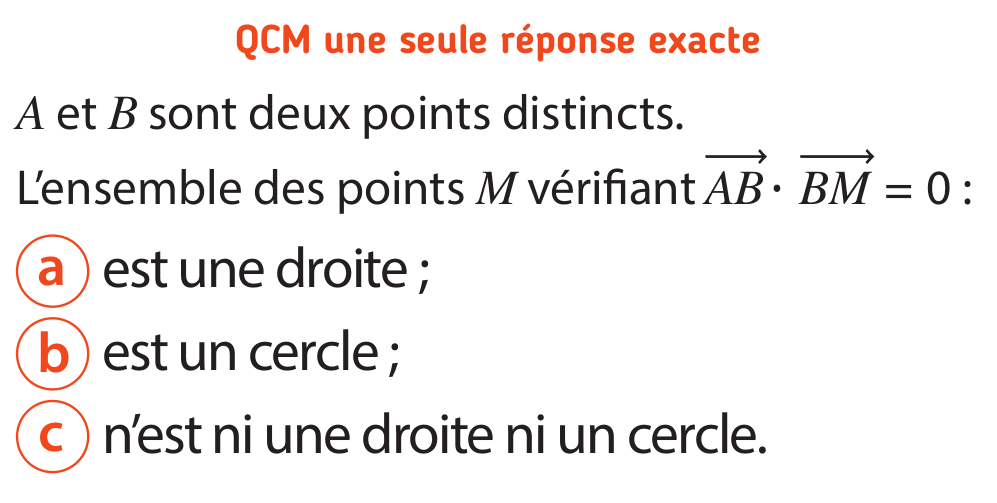
\includegraphics[scale=0.3]{ressources/prodscal-7.png}
\end{center}


\end{frame}



\begin{frame}
\automatisme{Application du produit scalaire}

\begin{center}
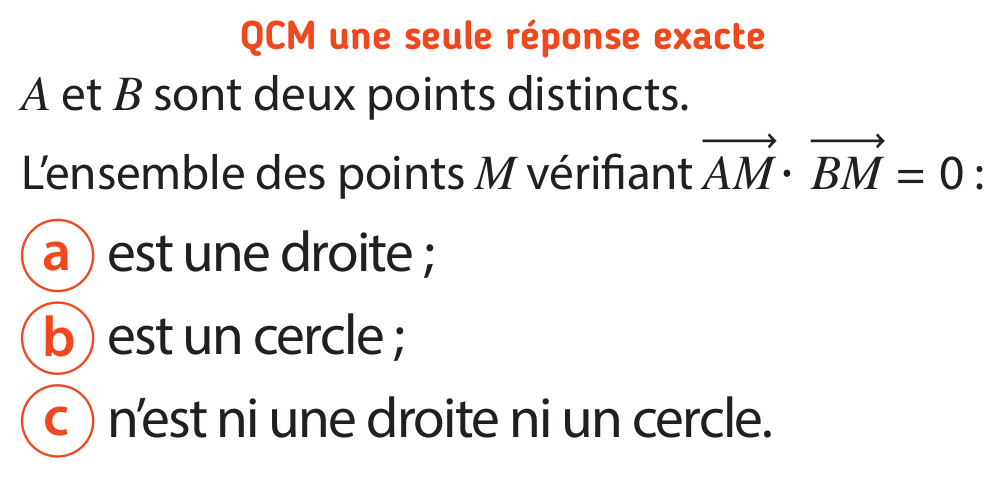
\includegraphics[scale=0.3]{ressources/prodscal-8.png}
\end{center}


\end{frame}







\end{document}